\chapter{Higgs Combinations and Properties}
\label{chap:combinations}

\section{Combined Higgs Searches}
\label{sec:combinations}

$\approx$ 3 pages results from sub-combiations, full combination, discovery

The likelihood is coded using \texttt{RooFit} version \texttt{5.3.0} under the 
\texttt{CMSSW} package \\
\texttt{HiggsAnalysis/CombinedLimit}%~\cite{combinationstwiki}.

\subsection{Diagnostics}

Frequentest statistical techniques often involve generating many pesudo-datsets (toys)
in order to build the distribution of a test-statistic. As described in Chaper~\ref{chap:hgg},
these distributions are used to set confidance intervals or determine the significance of
some observed excess in experimental data. The combined Higgs searches at CMS employs the
profiled likelihood test-statistic (Equation~\ref{eqn:llr}) in which the nuisance parameters,
$\boldth$, are profiled (fit) from the data. 
For calculating the significance of an excess in data, the distribution
of the test-statistic $q_{0}$ under the background only hypothesis is required. 
The procedure for determining this distribution proceeds as follows;

\begin{itemize}
\item{Fit the observed data fixing $\mu=0$. The values of the nuisance parameters 
at which the likelihood attains its maximum are denoted $\boldth_{obs}$ and will represent 
the expectation value of the nuisance parameters in the likelihood.}
\item{Generate a toy dataset under the background only hypothesis. For the purposes of
generating data, the nuisance parameters are fixed to $\boldth=\boldth_{obs}$.}
\item{Fit the toy dataset twice, once fixing $\mu=0$, $\call(data|0,\hat{\boldth}_{0})$ 
and once more letting 
$\mu$ float freely, $\call(data|\hat{\mu},\hat{\boldth})$. When 
evaluating the likelihood, the values $\boldth_{obs}$ are re-generated in order to 
model the systematic uncertainties.}
\end{itemize}
Around 10,000 toys were generated and fitted under this procedure. The distributions
of the values of the nusiance parameters from each fit are used to diagnose the fits 
and highlight potentially problematic channels entering the combination~\cite{AN-12-317}.
Figure~\ref{fig:combination_cmsefft} is a summary of the results for the nuisance parameter, \texttt{CMS\_eff\_t}, 
which models the systematic associated to the uncertainty on the efficiency to reconstruct tau-leptons.
The upper left panel shows two pull distributions of the values from the fit defined as the difference between 
the value of the fitted parameter and the value from the best fit to data, $\boldth_{obs}$, 
divided by the $1\sigma$ uncertainty on the parameter before fitting to the data. 
The blue histogram includes all toys while the red shows the results
only for which the best fit signal strength is positive. Since the test-statistic $q_{0}$ is designed 
to report only excesses in the data, it is important to check that nuisance parameters correlated to 
the signal strength are well-behaved. The pull distributions are fitted with a Gaussian and the width and mean 
are reported in the upper right panel. Since the constrain terms in the 
likelihood for nuisances are generated around the best fit to data, the pulls are expected to be centered 
around 0. For this nuisance parameter, the width of the pull distribution is less than unity, indicating
that the data are able to constrain this parameter. This is reflected in the lower left panel 
which shows little correlation between the nusiance parameter and the value generated for the expectation
of this parameter (\texttt{CMS\_eff\_t\_In}) in each toy. Nuisances which are constrained by the data can indicate that an
uncertainty has been over-estimated. However, this particular parameter is correlated across several
channels. The constraint is likely due to the fact that this parameter effects a background process
in one decay channel and the signal in another.


The lower right panel shows the shape of the negative log-likelihood (NLL) as a function of the 
nuisance parameter near its minimum. At each point, all other parameters are fixed 
to those of the best fit to the data (in this case, from the fit allowing $\mu$ to float).
The likelihood is expected to be parabolic around its minima with no secondary (local) minima present.
Degenerate minima, which can cause instabilities in the fitting procedure, will be visible in the 
shape of the negative log-likelihood.


\begin{figure*}[hbtp]
  \begin{center}
    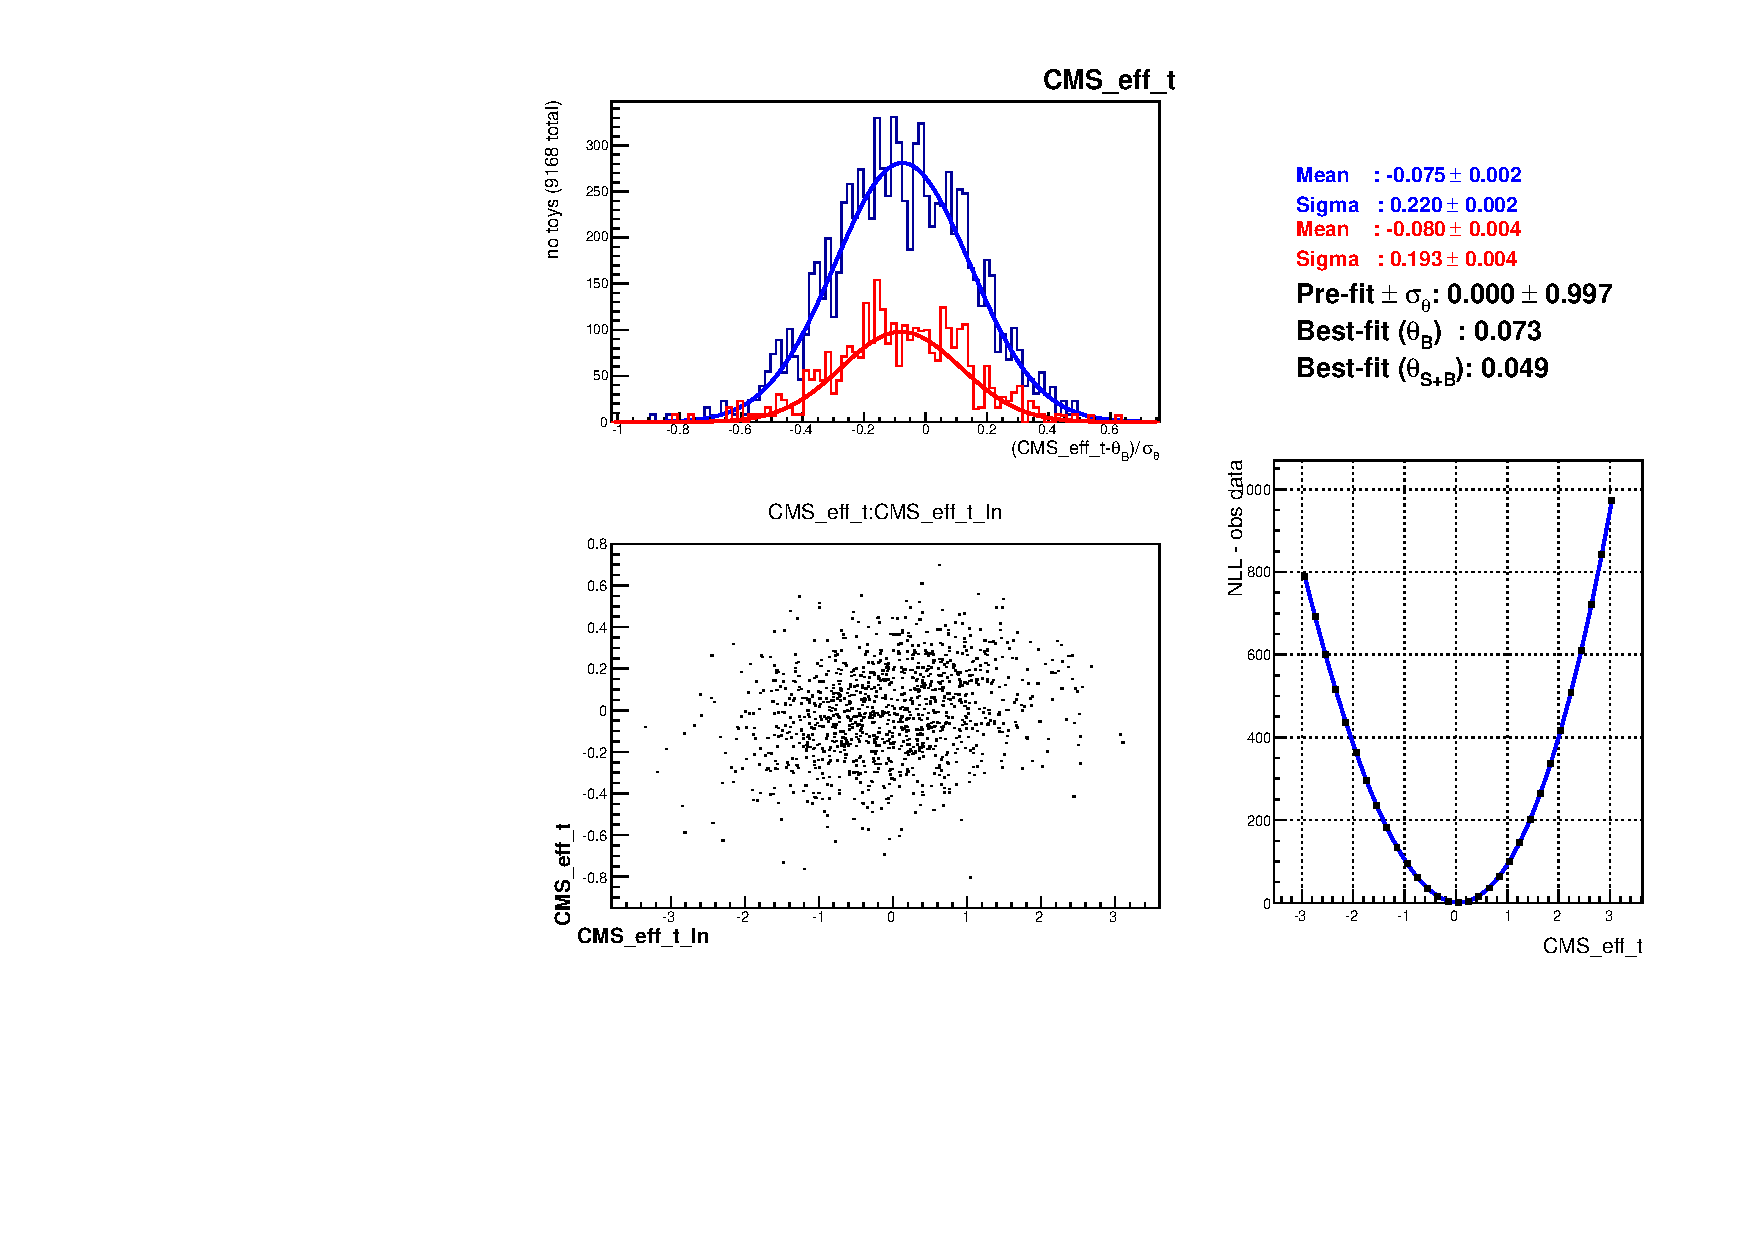
\includegraphics[width=\textwidth]{combinations/diagnostics/tree_fit_sb_CMS_eff_t.pdf}
    \caption{Summary plots for the parameter \texttt{CMS\_eff\_t}. 
	The entries in the histograms are for fits to toys generated under the background only
	hypothesis letting $\mu$ float freely. The bottom, left panel shows the correlation
	between the value generated for the expectation value of the nuisance \texttt{CMS\_eff\_t} 
	and the fitter value of the parameter. The lower right panel shows the shape of the 
	negative log-likelihood (NLL) as a function of the nuisance parameter.}
    \label{fig:combination_cmsefft}
  \end{center}
\end{figure*}


\subsection{Combination Results}


